\documentclass[norsk,a4paper]{article}
% Setter orddelingsregler for norsk (se opsjon "norsk" over)
\usepackage{babel}
% Setter UTF-8 tegnsett for latex (et passende utvalg fra Unicode for norsk)
\usepackage{ucs}
\usepackage[utf8x]{inputenc}
\usepackage[T1]{fontenc}
\usepackage[hidelinks]{hyperref}
\PreloadUnicodePage{0}
% Håndterer mellomrom på en smidig (og automatisk) måte.
\usepackage{xspace}
% Gjør lenker (også internt i dokumentet) klikkbare
\usepackage{hyperref}
% God formatering av URL
\usepackage{url}
% Gjør farger tilgjengelig, feks fargede bokstaver og strektegninger
\usepackage{color}
% Kommandoer for å integrere bilder i teksten
\usepackage{graphicx}
% Justering av margene (mindre enn standard oppsett)
\usepackage[hmargin=3.5cm,vmargin=2.7cm]{geometry} 
% Endring av undertekst til bilder
\usepackage{caption}


% Tittel, forfatter(e)
\title{Matkrig}
\author{Tony H. Abaz, Eirik Rye Ahlsen, Emilia Botnen}
\date{}



\begin{document}
% Legger tittelen først i dokumentet
\maketitle
\date{}
% Lager en innholdsfortegnelse - kommentert ut
% \tableofcontents
% Starten på selve teskten

\section*{Introduksjon}
Matkrig er et 2D-platform strategi artilleri spill som går ut på å skyte mat på motstanderen. Spilleren har kontroll  over en spillfigur og har tilgang til simple bevegelighets mekanismer. Spillet er delt inn i to faser; Bevegelsesfase hvor alle spillerene kan bevege seg i heltid, og en skytefase hvor spillerene kan skyte hverandre. Målet med spillet er å være den siste som gjenstår på banen, og spilleren kan oppnå dette ved hjelp av å skade motstanderene helt til de er tom for livspoeng. Målgruppe kan være alle aldre, men vil vel kanskje appellere mest til barn/ungdom. Det vil ikke kreve noen spesifikke kunnskaper for spillet. En spillerunde er ikke fast satt, bestemmes ut ifra hvor fort eller sakte spilleren spiller. En runde skal maksimalt vare i 15 minutter. Det skal være mulig å lagre spillet underveis for så å gjenoppta det på et senere tidspunkt. Det vil bare være en spillrunde. Spillet skal kunne spilles mot både datamaskin og andre spillere. Åpne data som skal brukes er fra matvaretabellen: \url {https://www.europeandataportal.eu/data/en/dataset/http---data-norge-no-node-493}



\tableofcontents


\newpage
\section{Spilleregler}
Spillet begynner med at spilleren kan velge mellom å spille mot datamaskin eller andre spillere. Spilleren får i starten en sum penger for å kunne kjøpe ammunisjoner/mat. Spilleren får i starten bevege seg fritt i 10 sekunder, man kan flytte seg ved å gå og hoppe. Deretter får man 15 sek på å velge våpen, skyteretning, -lengde og -kraft. Alle angrepene utføres samtidig. Blir man truffet av mat mister man helsepoeng ut ifra skade. Når man er tom for helsepoeng taper man spillet, mister alle motstanderen alle helsepoengene sine vinner du spillet. Blir de siste tom for helsepoeng samtidig blir det uavgjort mellom dem. Om du og en eller flere av motstanderne fortsatt har helsepoeng gjentas bevegelse- og skytefasen helt til en vinner gjenstår.

\section{Hovedflyt}
\label{tips_tekst} % etikett det kan referes til

\textbf{\large{1.}}	Aktør får * sekunder på å bevege seg fritt på kartet. \\
\textbf{\large{2.}}	Aktør velger våpen \\
\textbf{\large{3.}}	Aktør velger retning \\
\textbf{\large{4.}}	Aktør velger kraft for lenge og skade \\
\textbf{\large{5.}}	Systemet registrer prosjektilposisjon \\
\textbf{\large{6.}}	Systemet endrer miljøet ut ifra prosjektilkraft og type \\
\textbf{\large{7.}}   Motstander blir truffet av prosjektil \\
\textbf{\large{8.}}  Systemet beregner skade. \\
\textbf{\large{9.}}  Motstander mister helsepoeng \\
\textbf{\large{10.}} Motstander dør \\
\textbf{\large{11.}} Gjenstående spiller vinner \\	

\textbf{\large{}}\\
\textbf{\large{A1. @1 	}}Aktør beveger seg ut av kartet \\
\textbf{\large{A2. 		}} Gjenoppta @11\\
\\
\textbf{\large{B1. @2 }} Aktør har ikke ammunisjon\\
\textbf{\large{B2. }} Gjenoppta @2\\
\\
\textbf{\large{C1. @9 }} Motstander overlever\\
\textbf{\large{C2.}} Gjenoppta @1\\
\\
\textbf{\large{D1. @Everywhere	}}  Tiden går ut \\
\textbf{\large{D2. }}Aktør med mest gjenstående helsepoeng vinner.\\
\\
\textbf{\large{E1. @2}} Tid for å velge våpen/retning/kraft går ut \\
\textbf{\large{E2.}} Aktør får ikke angrepet \\
\textbf{\large{E3.}} Gjenoppta @1 \\

\newpage





\section{Brukerhistorie}


\begin{center}
    \begin{tabular}{ | p{5.5cm} | l | l |}
    \hline
   \textbf{\large Brukerhistorie} & \textbf{\large Funksjonell/ikke-funksjonell} & \textbf{\large Skal ha/burde ha}\\ \hline
   Som en bruker, vil jeg ha en spillmeny,sånn at jeg kan velge hvem jeg skal spille mot. & funksjonell & skal ha   
    \\ \hline
    Som en bruker, vil jeg ha mulighet for å velge karttema(farger, terreng), sånn at det blir variasjon i spillet. & ikke-funksjonell & burde ha 
     \\ \hline
    Som en bruker, vil jeg ha mulighet for å velge tilfedlig generete kart, sånn at det blir variasjon i spillet. & ikke-funksjonell & burde ha
    \\ \hline
    Som en bruker, vil jeg hoppe med spillfiguren, sånn at figuren kan komme seg over hindringer/hull. & funksjonell & skal ha
    \\ \hline
    Som en bruker, vil jeg ha helsepoeng på spillfiguren, sånn at spillfiguren ikke taper med en gang. & funksjonell & skal ha
    \\ \hline 
    Som en bruker, vil jeg velge et våpen hver skytefase, sånn at jeg kan skade motstanderen. & funksjonell & skal ha
  \\ \hline
  Som en bruker, vil jeg ha en skytefase sånn at jeg kan ha mulighet for å skade motstanderen. & funksjonell & skal ha
  \\ \hline
  Som en bruker, vil jeg ha en bevegelsesfase sånn at jeg kan finne en god posisjon for skytefasen. & funksjonell & skal ha
  \\ \hline
  Som et bruker, vil jeg at at det skal veksles mellom bevegelsesfase og skytefase. & funksjonell & skal ha
  \\ \hline
  Som en bruker, vil jeg kunne gå frem og tilbake sånn at jeg kan bevege meg i bevegelsesfasen. & funksjonell & skal ha
  \\ \hline
 Som en bruker, vil jeg kunne kjøpe ammunisjon sånn at jeg kan angripe motstanderen med forskjellige våpen. & funksjonell & skal ha
 \\ \hline
 Som en bruker, vil jeg kunne ha tilgang til en våpenbutikk sånn at det blir oversiktlig å kjøpe ammunisjon. & ikke-funksjonell & skal ha.
 \\ \hline
 Som en bruker, vil jeg at de forksjellige fasene skal ha en spesifisert varighet. & ikke-funksjonell & skal ha
 \\ \hline
 Som en bruker, vil jeg at en spillfigur taper når helsepoeng blir 0. & funksjonell & skal ha
  \\ \hline
  Som en bruker, vil jeg at våpenskade skal bestemmes av åpen data om kaloriinnhold for den korrisponderende maten i våpenet sånn at spillet får et særpreg. & funksjonell & skal ha
  \\ \hline
  Som en bruker, vil jeg at spillet avsluttes når det kun er en spiller igjen med helsepoeng. & funksjonell & skal ha
  \\ \hline
 
  
    \end{tabular}
\end{center}

\newpage




% Inkludere en annen latex-fil som en del av dette dokumentet.
%\input{hjelpefil}

%%%%%%
\section{Skisser}
\begin{figure}[!htb]
% \includegraphics[width=0.98\textwidth]{ctan_lion_600.png}

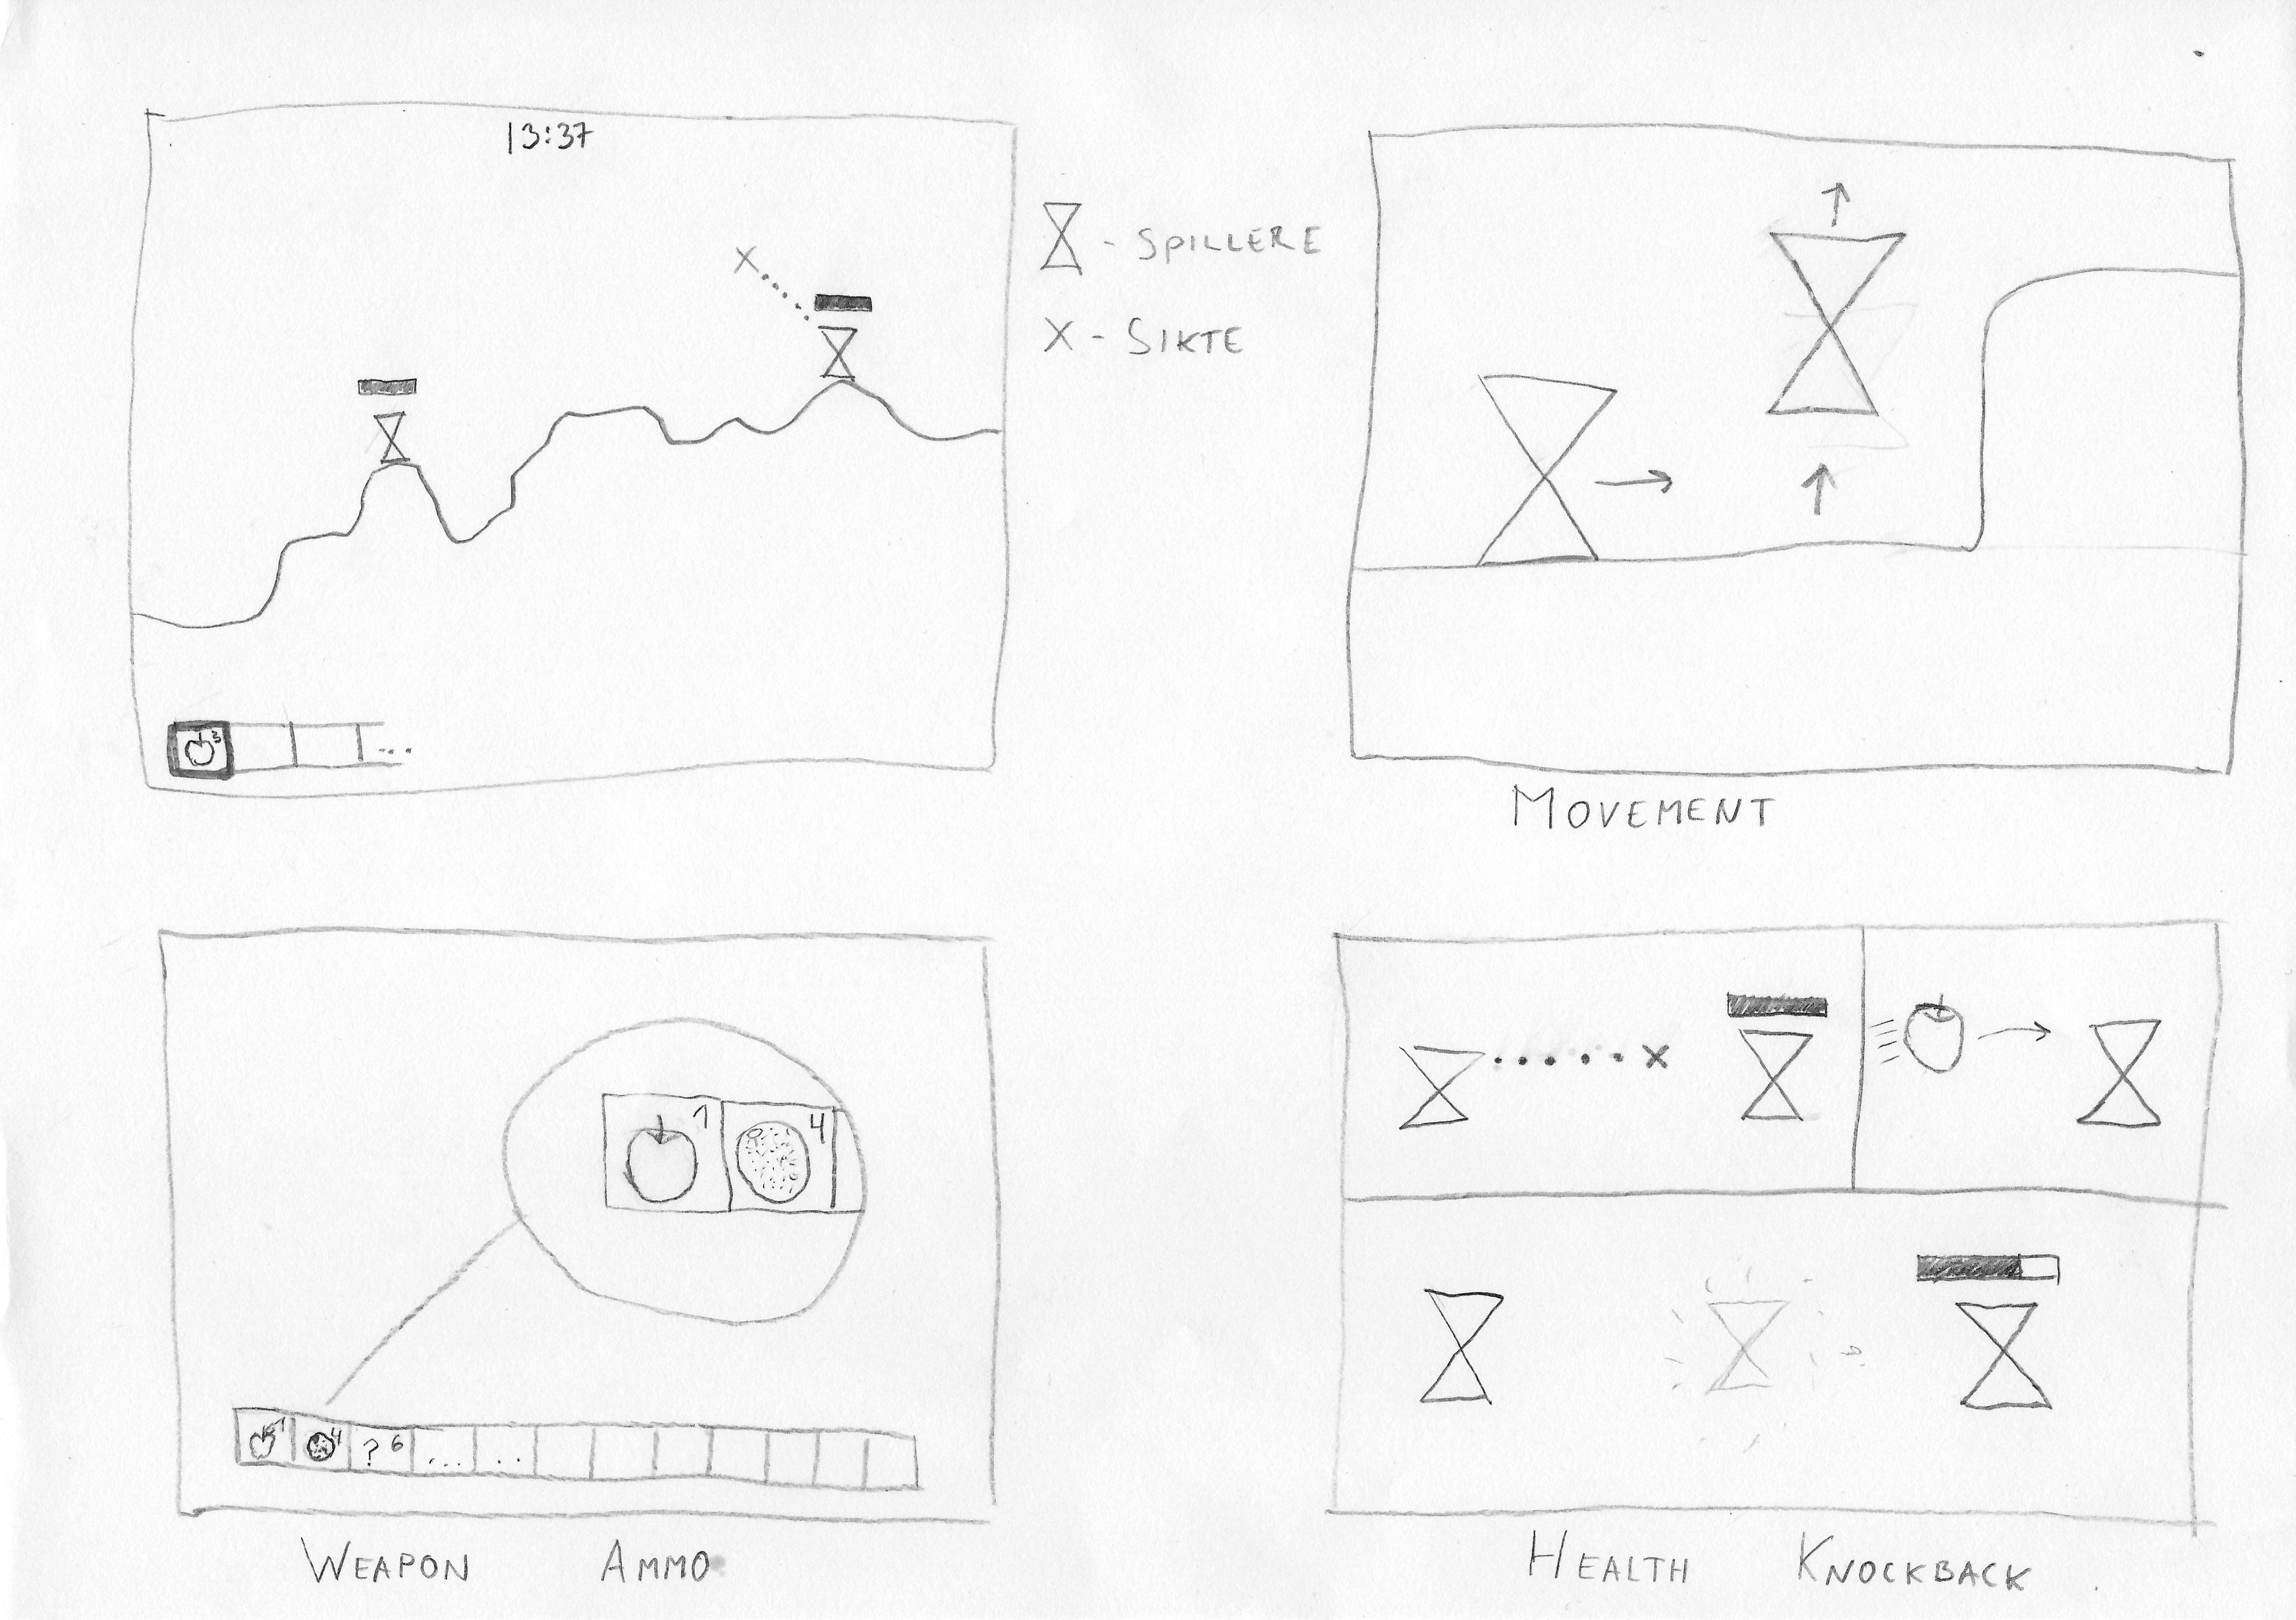
\includegraphics[width=1\textwidth]{Skisse_01.jpg}
%\caption{ }
%\caption{CTAN lion drawing by Duane Bibby (fra \url{https://www.ctan.org/lion/files}).}


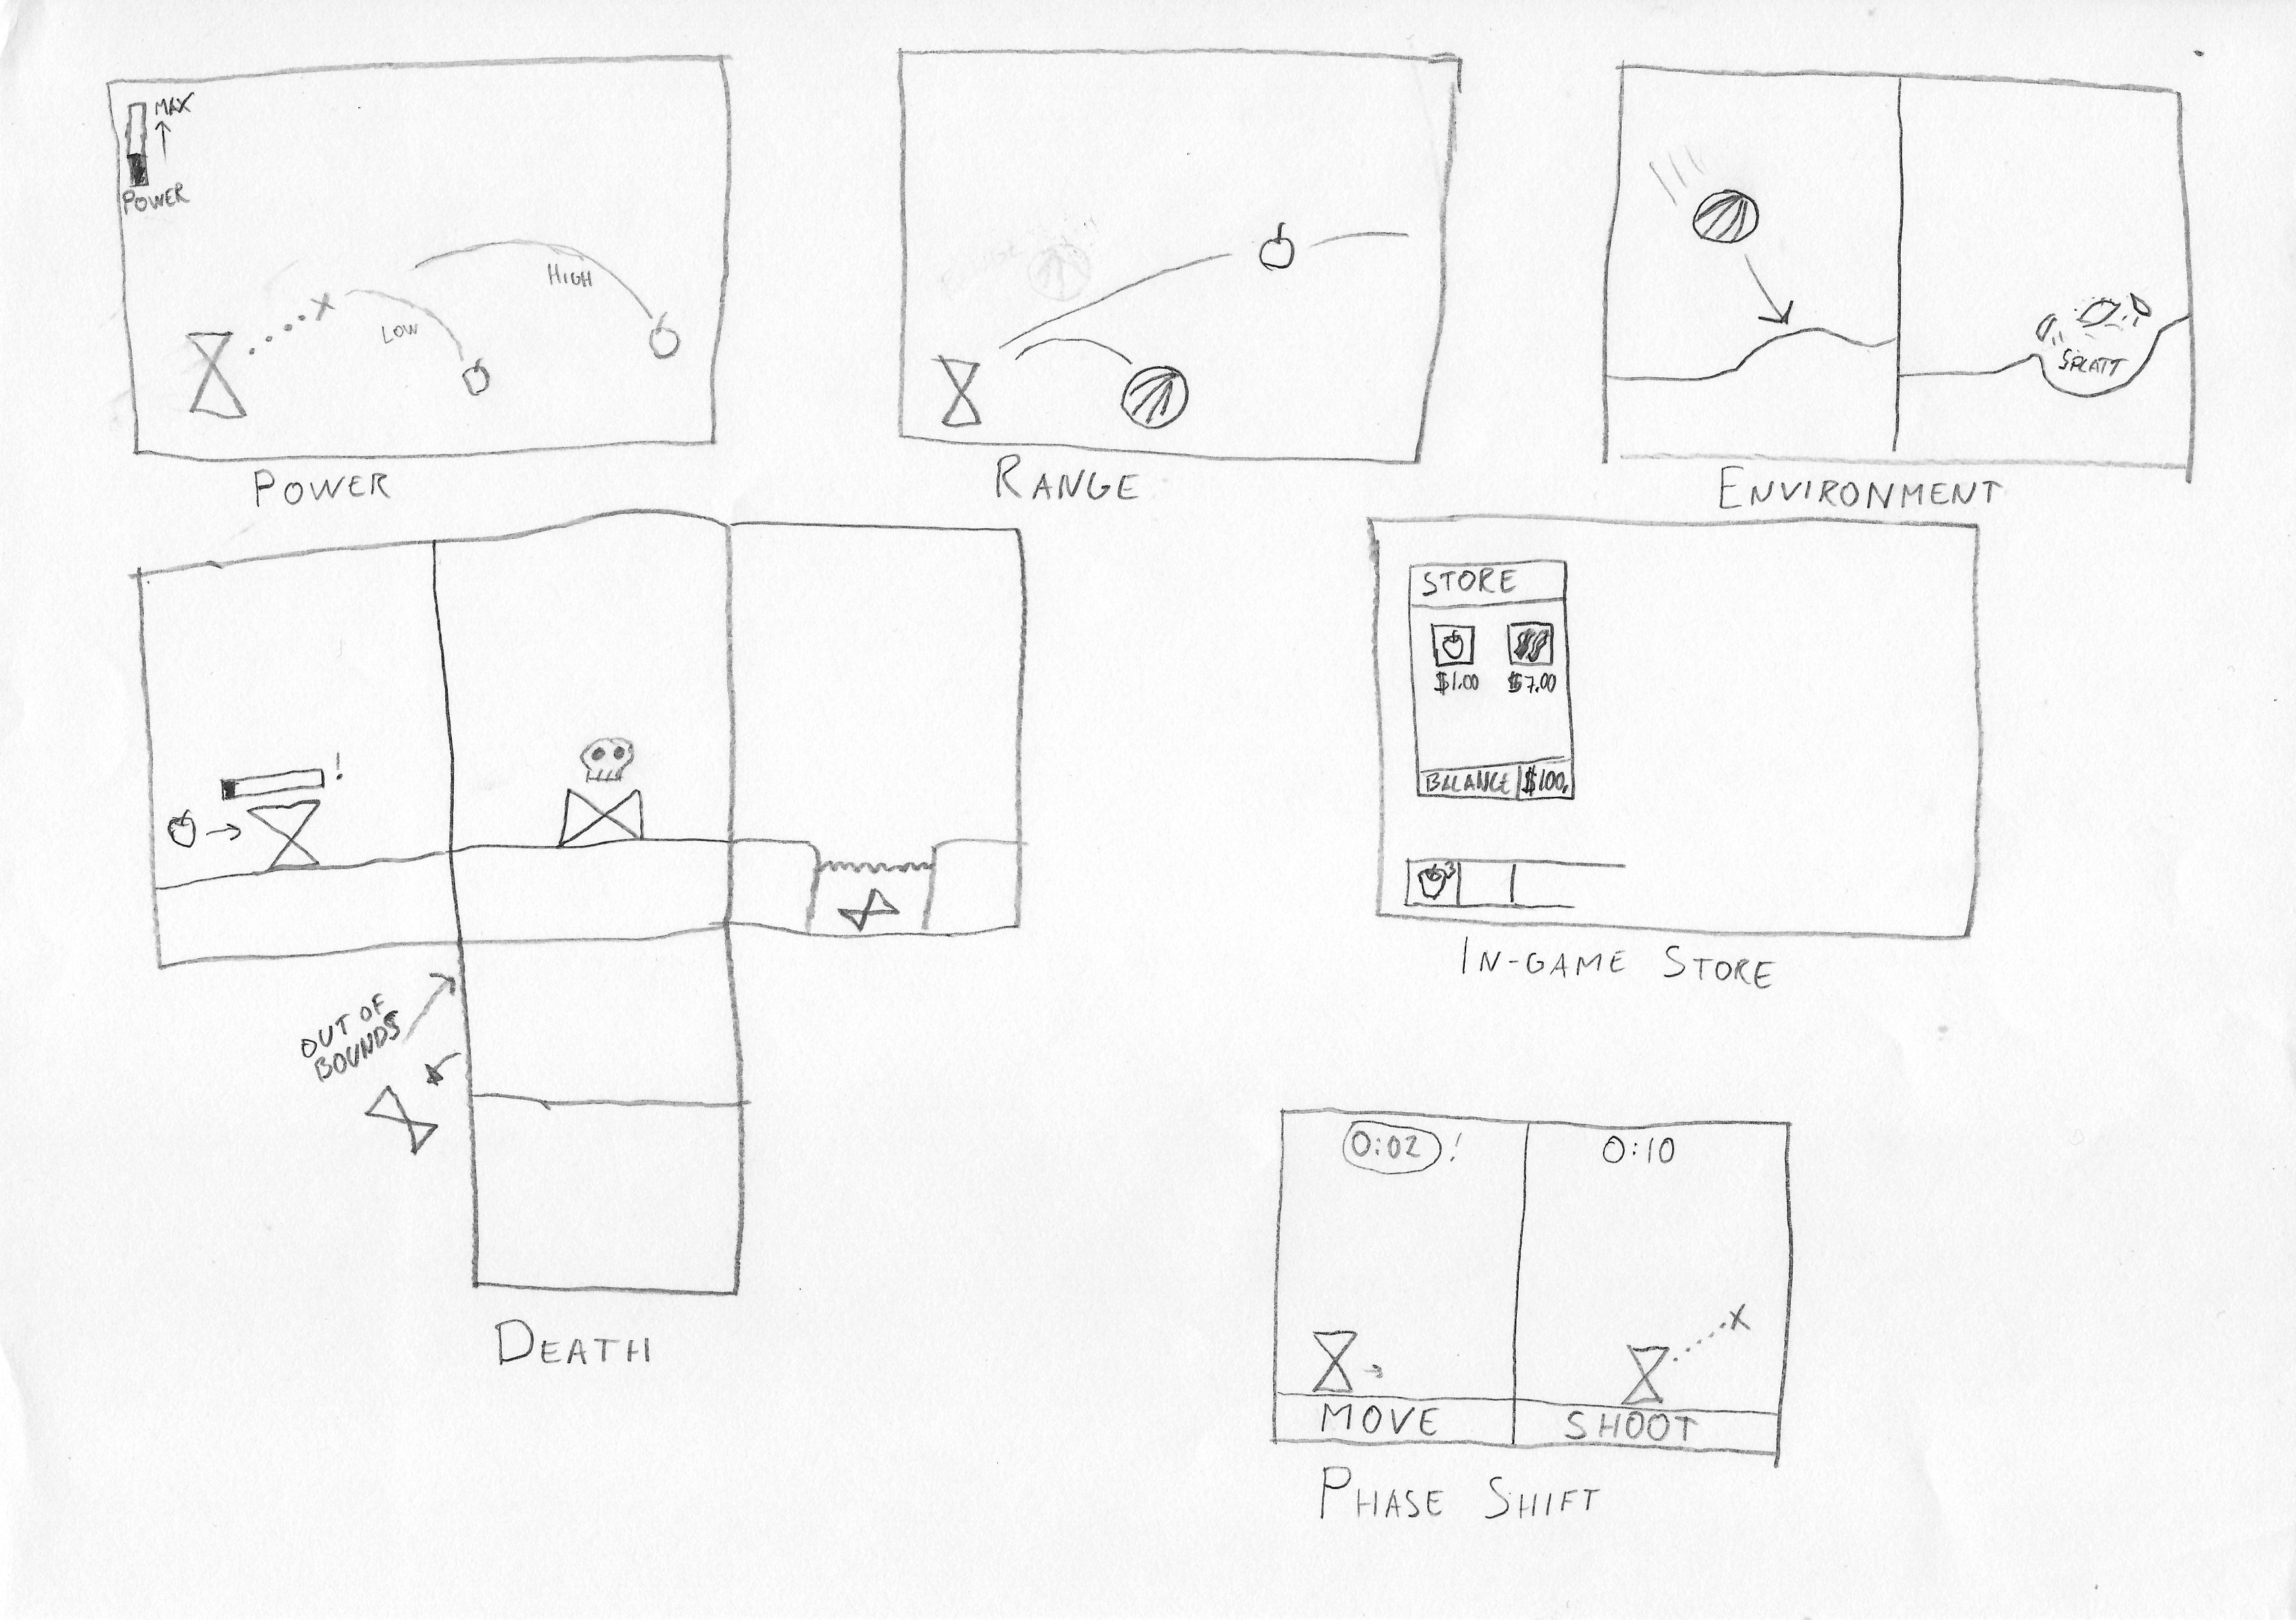
\includegraphics[width=1\textwidth]{Skisse_02.jpg}
%\caption{}
%\label{}
%\label{ctan_lion}
\end{figure}



\newpage
\section{Diagram}
\begin{figure}[!thb]
\centering
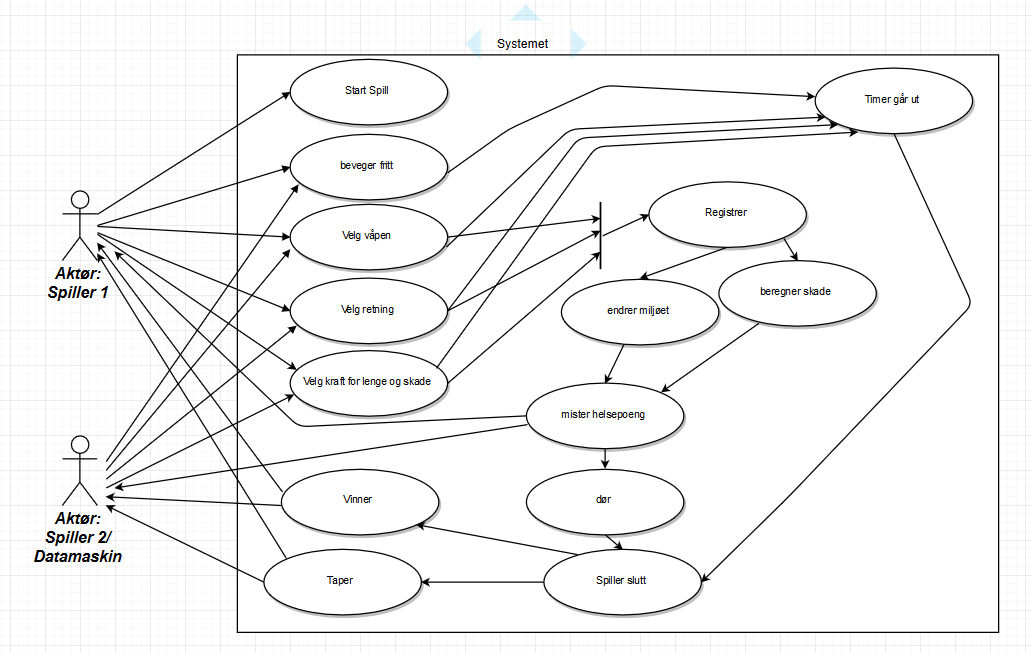
\includegraphics[width=1\textwidth]{uml_diagram.png}
\captionsetup{labelformat=empty}
\caption{Et eksempelspill med to spillerere}
\end{figure}



\end{document}
